\section{Introduction}
\label{sec:intro}


% Recent advances in deep learning have significantly improved object detection. However, these data-driven models can inherit or amplify biases from training datasets, leading to poor transferability across domains~\cite{mehrabi2021survey}.
% To address these challenges, researchers have explored various techniques [ref] to enhance the robustness and generalization capabilities of deep learning models. 
% One promising technique is domain generalization~\cite{blanchard2011generalizing} (DG),
% which aims to learn a model from one or multiple source domains that can perform well on out-of-distribution (OOD) target domains. 
% Existing mainstream DG methods primarily focus on learning domain-invariant representations~\cite{li2018deep,rahman2020correlation,albuquerque2019generalizing,deng2020representation}, expanding source distributions through data augmentation~\cite{tobin2017domain,peng2018sim,xu2021fourier,zhou2021domain}, or leveraging the strong prior knowledge of Vision Foundation Models (VFMs) ~\cite{wei2024stronger,yun2025soma,he2025generalized,he2025boosting}.



% Recent breakthroughs in deep learning have substantially advanced the accuracy and efficiency of object detection systems across a wide range of applications. 
% Despite these achievements, 
Despite recent advances, data-driven object detection models often inherit or amplify dataset biases, limiting their cross-domain transferability~\cite{mehrabi2021survey}. 
They frequently perform poorly across diverse viewpoints and imaging conditions from ground-level scenes to aerial imagery, which hinders generalization.
% For instance, detectors trained on standard datasets may struggle when applied to remote sensing imagery, such as UAV images captured under different weather conditions, where variations in illumination and scene appearance can dramatically alter object visibility. 
\begin{figure}[t]
    \centering
    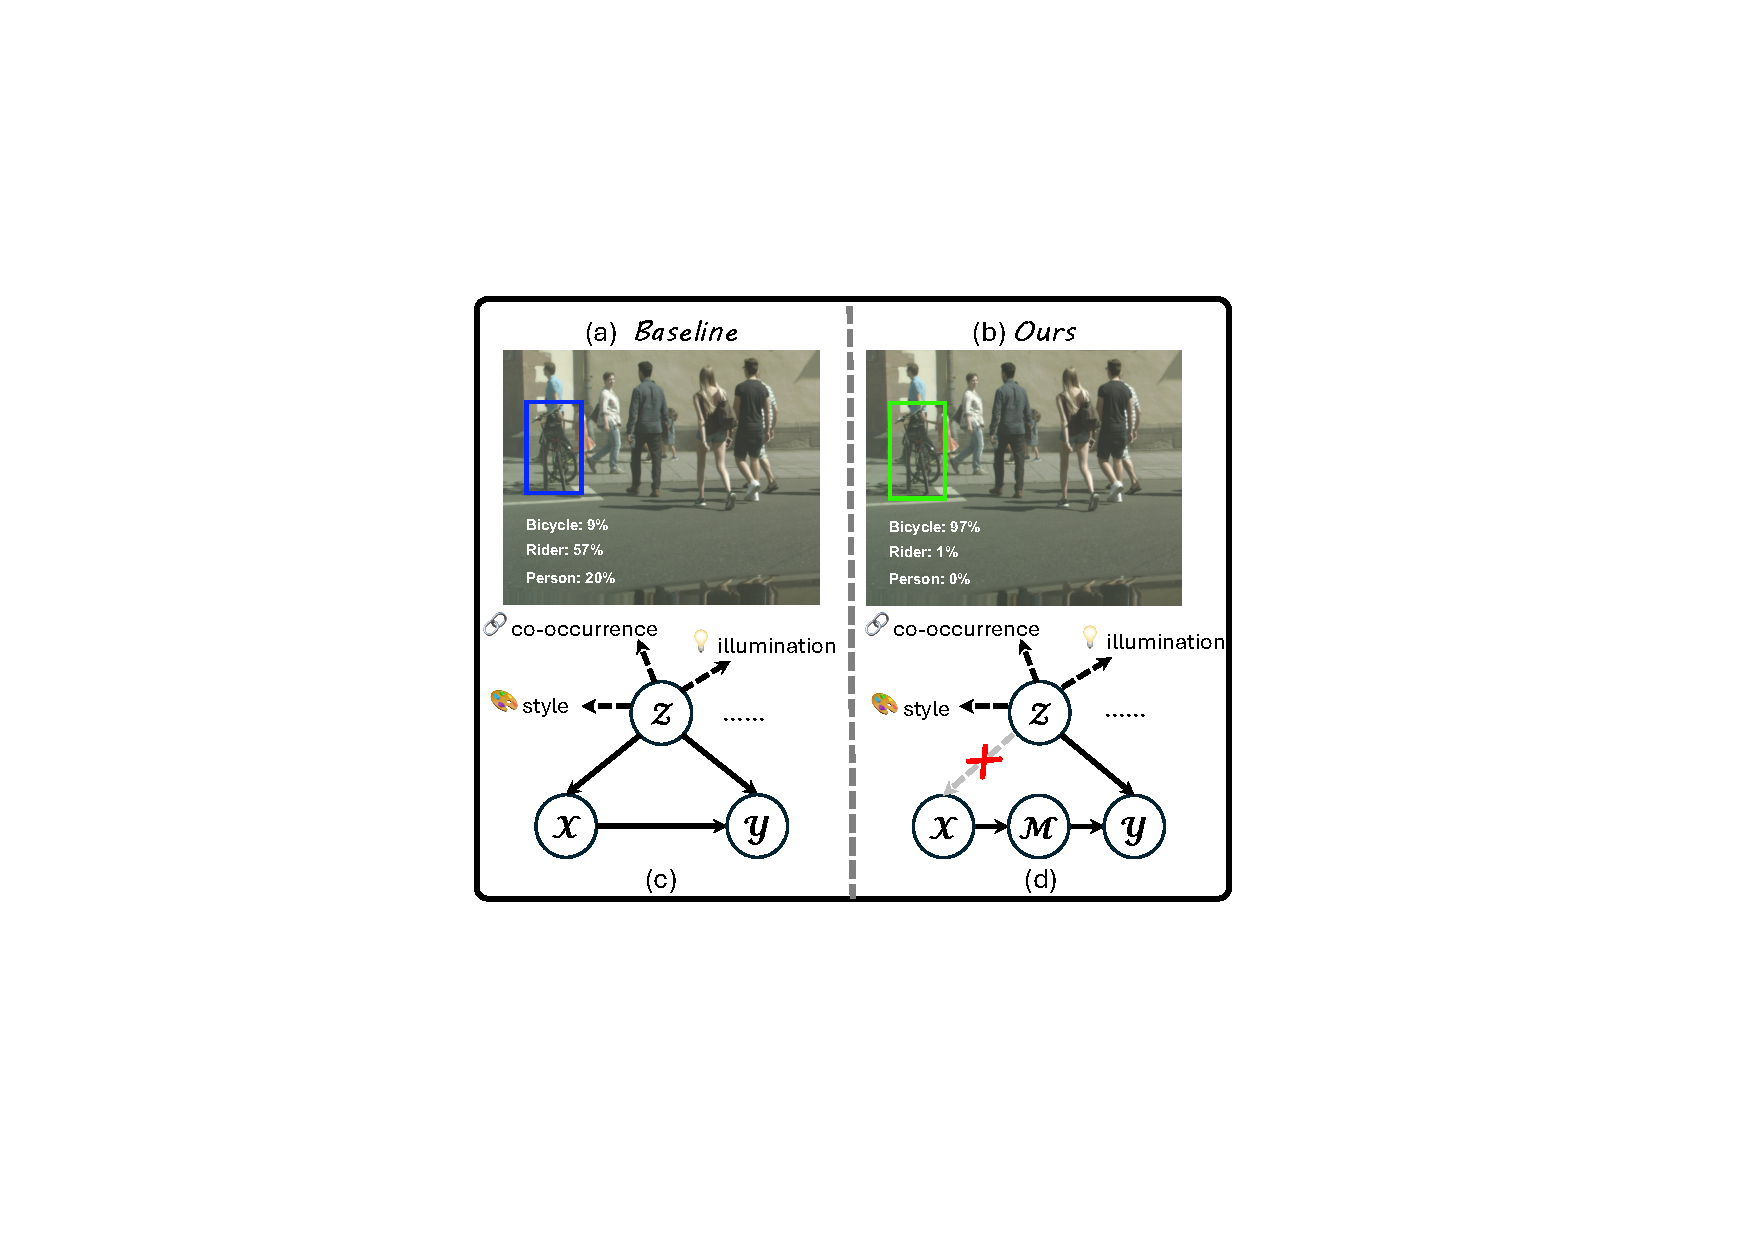
\includegraphics[width=0.47\textwidth]{figs/teaserv2.pdf}
    \caption{
(a) The baseline model, using a frozen DINOv2~\cite{oquab2023dinov2} backbone, misclassifies the object due to spurious correlations caused by the confounder: co-occurrence of a bicycle with nearby pedestrians.
(b) Our method correctly identifies the bicycle by blocking these spurious correlations.
(c) Models may rely on spurious correlations between the input $\mathcal{X}$ and the label $\mathcal{Y}$ through confounders $\mathcal{Z}$.
(d) In contrast, our method implements a front-door adjustment mechanism, where the mediating variable $\mathcal{M}$ mitigates the influence of spurious correlations induced by $\mathcal{Z}$, thereby enabling the model to focus on the features that truly determine $\mathcal{Y}$.
}
    \label{fig:teaser}
    \vspace{-5mm}
\end{figure}

To address these limitations, domain generalization (DG)~\cite{blanchard2011generalizing} has emerged as a particularly promising paradigm, aiming to train models on one or multiple source domains to generalize effectively to unseen out-of-distribution (OOD) target domains. 
Existing DG approaches primarily focus on learning domain-invariant representations~\cite{li2018deep,rahman2020correlation,albuquerque2019generalizing,deng2020representation}, expanding source distributions through data augmentation~\cite{tobin2017domain,peng2018sim,xu2021fourier,zhou2021domain}, or leveraging the strong prior knowledge embedded in Vision Foundation Models (VFMs)~\cite{wei2024stronger,yun2025soma,he2025generalized,he2025boosting}.

However, many DG approaches often neglect the confounding effects that arise from limited single-domain datasets. 
These confounders (denoted as $\mathcal{Z}$), including variations in illumination, co-occurrence patterns, or stylistic discrepancies, can bias the learned representations ($\mathcal{X}$) and create spurious correlations with object labels ($\mathcal{Y}$), see Fig.~\ref{fig:teaser}.
Such biases distort the causal link between visual features and labels~\cite{wang2020visual,zhang2022multiple,zhang2020causal,shao2021improving}, degrading out-of-distribution generalization.
For instance, a detector with a frozen DINOv2~\cite{oquab2023dinov2} backbone pretrained on \textit{142M} images but fine-tuned on only \textit{3,000} Cityscapes samples~\cite{cordts2016cityscapes} may misclassify a bicycle near a person as a rider (57\%) or even as a person (20\%) due to spatial correlations (Fig.~\ref{fig:teaser}~(a)).
The backbone offers substantial representational strength, yet overlooking spurious correlations in downstream tasks risks wasting much of this capacity.
Hence, to mitigate these effects, it is crucial to uncover and model the causal mechanisms behind the data, guiding the model to focus on causally relevant features rather than spurious correlations.





% However, most of these approaches overlook potential confounders inherent in limited single-domain datasets.  
% For example, consider a model with a frozen DINOv2~\cite{oquab2023dinov2} backbone, 
% pretrained on \textit{142M} images, whose object detection head is fine-tuned on Cityscapes~\cite{cordts2016cityscapes}, 
% which contains only around \textit{3,000} images. 
% This large discrepancy in data scale may induce spurious correlations in the trainable components, 
% potentially leading to misclassifications.  
% As illustrated in Fig.~\ref{fig:teaser}~(a), due to spatial correlation, the model misclassifies a bicycle located near a person standing behind it, 
% assigning it 57\% confidence as a rider and 20\% as a person.


% Real-world datasets generally contain various confounding factors (denoted as $\mathcal{Z}$), such as variations in illumination, co-occurrence patterns, or object styles, 
% which can bias the learned representations ($\mathcal{X}$) and produce spurious correlations with object labels ($\mathcal{Y}$). 
% When variations of these confounders are unbalanced in the datasets, they ultimately impair out-of-distribution generalization.
% To mitigate the adverse effects of these confounders, it is crucial to uncover the inherent causality underlying the data, thereby preventing the model from relying on spurious correlations.
% Real-world datasets inherently contain confounding factors~\cite{wang2020visual,zhang2022multiple,zhang2020causal,shao2021improving} that distort the causal relationship between visual features and object labels.
% These confounders (denoted as $\mathcal{Z}$), including variations in illumination, co-occurrence patterns, or stylistic discrepancies, can bias the learned representations ($\mathcal{X}$) and create spurious correlations with object labels ($\mathcal{Y}$), thereby undermining out-of-distribution generalization. 
% To mitigate these effects, it is crucial to uncover and model the causal mechanisms underlying the data, guiding the model to focus on causally relevant features rather than superficial correlations.




% In this context, we introduce \textbf{Bridge}, a novel \textbf{B}asis-\textbf{dr}iven causal inference framework for \textbf{D}omain \textbf{Ge}neralization, which incorporates causal inference~\cite{pearl2016causal,neuberg2003causality} into the object detection task to enable the model to learn inherent causal structures and mitigate the influence of confounders.
In this paper, we introduce \textbf{\textit{Bridge}}, a \textbf{B}asis-d\textbf{ri}ven framework for \textbf{D}omain \textbf{Ge}neralization that incorporates causal inference~\cite{pearl2016causal,neuberg2003causality} into object detection. 
% By uncovering intrinsic causal structures, 
By blocking the adverse effects of confounders,
\textbf{\textit{Bridge}} enables the model to mitigate the influence of confounders.
% Specifically, we propose a novel Causal Basis Block (CBB) that learns a front-door adjustment from a basis-learning perspective to mitigate the adverse effects of confounders~\cite{pearl2018book}.
Specifically, we propose a novel Causal Basis Block (CBB) that is designed in accordance with the front-door adjustment~\cite{pearl2018book}, formulated from a basis-learning perspective to mitigate the adverse effects of confounders.
Unlike prior works~\cite{wang2024vision,liang2024confounded,zhang2022multiple,zhang2020causal} that depend on external confounder dictionaries or involve elaborate post-processing mechanisms (e.g., clustering~\cite{zhang2020causal}, momentum updates~\cite{liang2024confounded}) with limited flexibility and scalability,
our CBB is proposed as an end-to-end, plug-and-play module tailored for VFMs-based object detection frameworks, allowing seamless integration while maintaining high flexibility and scalability.
% our CBB is end-to-end and can be seamlessly integrated into existing object detection frameworks via plug-and-play.
In our design, we build the Domain Generalization Object Detection (DGOD) framework upon frozen VFMs by integrating the CBB to perform causal modeling, avoiding costly fine-tuning the whole network. 
By blocking spurious correlations (Fig.~\ref{fig:teaser}~(d)), the framework allows the model to focus on inherent causality, yielding more robust and generalizable representations for downstream tasks and improving performance (Fig.~\ref{fig:teaser}~(b)).


% Specifically, we draw inspiration from the front-door adjustment~\cite{pearl2018book} in causal inference, which employs the \textit{intervention}~\cite{pearl2018book} technique to mitigate the adverse effects of confounders. 
% Unlike prior works~\cite{wang2024vision,liang2024confounded,zhang2022multiple,zhang2020causal} that depend on external confounder dictionaries or involve elaborate post-processing mechanisms (e.g., clustering~\cite{zhang2020causal}, momentum updates~\cite{liang2024confounded}), which limit their flexibility and scalability.
% We propose a novel Causal Basis Block (CBB) that learns to implement the front-door adjustment from a basis-learning perspective.
% The CBB is an end-to-end, plug-and-play module that can be seamlessly integrated into existing object detection frameworks.
% In our design, we build the Domain Generalization Object Detection (DGOD) framework upon frozen Vision Foundation Models, integrating the CBB to perform causal modeling. By blocking spurious correlations (Fig.~\ref{fig:teaser}~(d)), the framework allows the model to focus on inherent causality, yielding more robust and generalizable representations for downstream tasks and improving performance (Fig.~\ref{fig:teaser}~(b)).

% Furthermore, considering the practical challenges in remote sensing, where object detection often faces diverse weather and visibility conditions, existing datasets lack dedicated domain generalization benchmarks for evaluating performance under such scenarios. 
% Furthermore, practical challenges in remote sensing emphasize the lack of systematic evaluation benchmarks for domain generalization under real-world conditions. 
% Existing aerial and UAV datasets rarely capture the full diversity of environmental factors such as lighting, haze, or precipitation.
% To bridge this gap, we extend the DroneVehicle dataset~\cite{sun2022drone} by annotating weather conditions and organizing the images into four scenarios: Clear, Dark, Foggy, and Extreme Dark, enabling comprehensive evaluation under varying environmental conditions and quantifying biases.

Furthermore, we notice that the commonly used benchmarks~\cite{cordts2016cityscapes,yu2020bdd100k,sakaridis2018semantic,everingham2010pascal,inoue2018cross,wu2022single} for DGOD lack diverse viewpoints and imaging conditions from the sky.
To compensate for the current benchmarks for a more comprehensive evaluation, we extend the DroneVehicle dataset~\cite{sun2022drone} by annotating weather conditions and organizing the images into four scenarios: Clear, Dark, Foggy, and Extreme Dark, enabling comprehensive evaluation under varying environmental conditions.% and quantifying biases.



% Most of these approaches rely on classic backbone networks, such as VGGNet~\cite{simonyan2014very}, MobileNetV2~\cite{sandler2018mobilenetv2}, and ResNet~\cite{he2016deep}, to improve model generalization. However, the recent advent of vision foundation models (VFMs) pre-trained on large-scale datasets has opened new avenues for DG, owing to their remarkable generalization and transferability across diverse downstream tasks.

% In the context of generative VFMs, works such as DDT~\cite{ddt}, GDD~\cite{he2025generalized}, and Boost~\cite{he2025boosting} leverage the generative power of Stable Diffusion~\cite{rombach2022high} to enhance generalization in object detection. In parallel, discriminative VFMs have also shown strong potential for DG. Specifically, Rein~\cite{wei2024stronger} and SoMA~\cite{yun2025soma}, built upon ViT-family vision foundation models (DINO~\cite{oquab2023dinov2}, SAM~\cite{kirillov2023segment}, etc.), employ parameter-efficient fine-tuning strategies to adapt large-scale pre-trained representations for domain-generalized semantic segmentation.

% Despite the promising generalization capabilities of VFMs, leveraging them on limited single-domain datasets remains challenging. For example, DINOv2, pretrained on \textit{142M} images, is often fine-tuned on datasets like Cityscapes, which contain only \textit{3,000} images from a single source domain. 
% Such scarcity can induce spurious correlations or biases in the downstream trainable head [ref], which may lead to misclassifications, 
% as shown in Fig. XXX (a). 
% Specifically, in real-world scenarios, biases can stem from a variety of factors, 
% including lighting conditions, weather changes, object styles, occlusions, and co-occurrence patterns. 
% While some confounders are observable, others are subtle and difficult to perceive. Unfortunately, such issues have been largely overlooked in prior studies on VFM-based DG.




% In this context, we introduce \textbf{\textit{Bridge}}, a novel \textbf{B}asis-d\textbf{ri}ven causal inference framework for \textbf{D}omain \textbf{Ge}neralization.
% \textbf{\textit{Bridge}} aims to bridge the gap between large-scale pretraining and specific downstream tasks, where models are often fine-tuned on limited, biased single-domain data.
% Motivated by the front-door adjustment~\cite{pearl2018book} in causal inference, \textbf{\textit{Bridge}} introduces a Causal Basis Block (CBB) that learns to implement the front-door adjustment, 
% mitigating spurious correlations that may arise from limited downstream data, via basis learning in the feature space.
% Specifically,
% by leveraging learnable \textit{Sample queries} and representing features in a low-rank basis, 
% \textbf{\textit{Bridge}} approximates the front-door adjustment directly in feature space without requiring external 
% confounder dictionaries or sequential post-processing, producing robust and generalizable representations for downstream tasks.
We summarize our main contributions as follows:
\begin{itemize}
\item We propose \textbf{\textit{Bridge}}, a novel framework that can be seamlessly integrated with both discriminative (e.g., DINOv2~\cite{oquab2023dinov2}, DINOv3~\cite{simeoni2025dinov3}, SAM~\cite{kirillov2023segment}) and generative (e.g., Stable Diffusion~\cite{rombach2022high}) Vision Foundation Models (VFMs), aiming to mitigate spurious correlations in downstream domain generalization object detection.
\item We introduce a novel Causal Basis Block that constructs front-door adjustments from a basis-learning perspective, which can be trained end-to-end and improves model generalization by producing robust representations.
\item We conduct extensive experiments on five DGOD benchmarks. 
\textbf{\textit{Bridge}} surpasses the previous runner-up across all the benchmarks by 
$\mathbf{+3.8}$, $\mathbf{+2.9}$, $\mathbf{+2.4}$, $\mathbf{+0.4}$, 
and $\mathbf{+1.5}$ in mAP, and consistently improves the VFMs (SAM, DINOv2, DINOv3) with average gains of 
$\mathbf{+2.7}$, $\mathbf{+4.5}$, $\mathbf{+3.1}$, $\mathbf{+1.8}$, 
and $\mathbf{+1.8}$ in mAP, respectively.

% \item We conduct extensive experiments on five domain generalization benchmarks, demonstrating that \textbf{\textit{Bridge}} consistently enhances robustness and generalization across both discriminative (SAM, DINOv2, DINOv3) and generative (Stable Diffusion) Vision Foundation Models, achieving average mAP gains of $\mathbf{+3.0}$, $\mathbf{+4.1}$, $\mathbf{+2.8}$, $\mathbf{+1.4}$, and $\mathbf{+1.8}$.
% Noteworthily, among the five benchmarks, we enrich an existing UAV object detection dataset with manually annotated weather condition labels, establishing a much-needed benchmark for evaluating domain generalization under diverse weather scenarios in the remote sensing community.
\item We enrich an existing UAV object detection dataset with manually annotated weather condition labels, establishing a much-needed benchmark for evaluating domain generalization under diverse weather scenarios in the remote sensing community.

\end{itemize}

